\documentclass[tikz,border=6pt]{standalone}

\usepackage{pgfplots}
\usepackage{xcolor}
\usepackage{scalefnt}

\usetikzlibrary{calc}

\pgfplotsset{compat=1.18}

% ============================================================
% Free parameters
% ============================================================

% Master font size for every textual element in the figure.
% Change only this value to resize axis ticks, right-axis labels,
% colorbar tick labels, and all other TikZ/PGFPlots text.
\def\PlotFontSize{14pt}
\newcommand{\PlotFont}{%
  \fontsize{\PlotFontSize}{\dimexpr 6\PlotFontSize/5\relax}\selectfont
}

% Analogs of ImageSize / AspectRatio
\def\PlotWidth{16cm}
\def\PlotHeight{10cm}

% Experimental-circle radius
\def\CircleRadius{5.0pt}

% Half-size of the theoretical x / + marker
\def\TheoryMarkerHalfSize{5.0pt}

% Thickness of the theoreti4al x / + marker
\def\TheoryMarkerLineWidth{1.15pt}

% Correspondence-arc style
\def\ArcLineWidth{1.15pt}

% WKB / quasiclassical-limit bars
\def\WKBHalfWidth{0.46}
\def\WKBOpacity{0.14}

% Experimental intensity range
\def\IntensityMin{-4.0}
\def\IntensityMax{0.0}

% Carrier frequency used for horizontal guide lines
\def\CarrierNu{0.309557114}

% Plot limits
\def\XMin{0.5}
\def\XMax{11.5}
\def\YMin{0.5}
\def\YMax{3.5}

% Plot colors
\colorlet{TheoryColor}{black}
\colorlet{ArcColor}{black!55}
\colorlet{GuideColor}{black!35}
\colorlet{WKBColor}{black}
\definecolor{IntensityLow}{RGB}{0,90,255}
\definecolor{IntensityHigh}{RGB}{255,65,20}

% ============================================================
% Data
%
% Theory:
%   m / n / nuTheory / boundFlag / matchedExperimentM / matchedExperimentN
%
%   boundFlag = 1 -> x
%   boundFlag = 0 -> +
%
%   matchedExperimentM / matchedExperimentN are retained in this data block
%   for compatibility, but correspondence arcs are now controlled by \ArcData
%
% Experiment:
%   m / n / nuExperiment / log10(intensity)
%
% IMPORTANT:
% Do not insert empty lines inside \TheoryData or \ExperimentData.
% ============================================================

\def\TheoryData{%
1/1/0.597710/0/0/0,%
1/2/1.396824/0/0/0,%
1/3/1.912467/0/0/0,%
1/4/2.310177/0/0/0,%
1/5/2.634192/0/0/0,%
1/6/2.917942/0/0/0,%
2/1/0.865299/0/0/0,%
2/2/1.523536/0/0/0,%
2/3/1.953101/0/0/0,%
2/4/2.310623/0/0/0,%
2/5/2.614279/0/0/0,%
2/6/2.885455/0/0/0,%
3/1/1.131266/0/0/0,%
3/2/1.623444/0/3/2,%
3/3/1.974809/0/3/3,%
3/4/2.300759/0/3/4,%
3/5/2.586529/0/3/5,%
3/6/2.846392/0/3/6,%
4/1/1.362948/0/4/1,%
4/2/1.702049/0/4/3,%
4/3/1.989035/0/4/4,%
4/4/2.285803/0/4/5,%
4/5/2.554147/0/4/6,%
4/6/2.802661/0/0/0,%
5/1/1.557260/0/0/0,%
5/2/1.758577/0/5/3,%
5/3/2.002209/0/5/4,%
5/4/2.268271/0/5/5,%
5/5/2.519518/0/5/6,%
5/6/2.756223/0/0/0,%
5/7/2.980032/0/0/0,%
6/1/1.703829/0/0/0,%
6/2/1.801624/0/6/3,%
6/3/2.019510/0/6/4,%
6/4/2.249405/0/6/5,%
6/5/2.484050/0/0/0,%
6/6/2.708482/0/0/0,%
6/7/2.923682/0/0/0,%
7/1/1.749139/1/0/0,%
7/2/1.881346/0/7/3,%
7/3/2.043832/0/0/0,%
7/4/2.232200/0/7/4,%
7/5/2.448722/0/7/5,%
7/6/2.660521/0/7/6,%
7/7/2.866267/0/0/0,%
8/1/1.727995/1/0/0,%
8/2/1.952073/1/0/0,%
8/3/2.075245/0/0/0,%
8/4/2.226939/0/8/4,%
8/5/2.414840/0/8/5,%
8/6/2.612834/0/0/0,%
8/7/2.811200/0/0/0,%
9/1/1.681505/1/0/0,%
9/2/1.964296/1/0/0,%
9/3/2.101770/1/0/0,%
9/4/2.245389/0/0/0,%
9/5/2.388427/0/0/0,%
9/6/2.570164/0/0/0,%
9/7/2.770481/0/0/0,%
9/8/2.991423/0/0/0,%
10/1/1.618404/1/0/0,%
10/2/1.929073/1/0/0,%
10/3/2.108371/1/0/0,%
10/4/2.256419/1/0/0,%
10/5/2.392629/0/0/0,%
10/6/2.548255/0/0/0,%
10/7/2.752192/0/0/0,%
10/8/2.982525/0/0/0,%
11/1/1.542436/1/0/0,%
11/2/1.865446/1/0/0,%
11/3/2.094002/1/0/0,%
11/4/2.246381/1/0/0,%
11/5/2.420872/0/0/0,%
11/6/2.560971/0/0/0,%
11/7/2.751976/0/0/0,%
11/8/2.984210/0/0/0%
}

\def\ExperimentData{%
3/1/1.2421/-1.681418437,%
3/2/1.5466/-1.874033745,%
3/3/1.8591/-1.687255777,%
3/4/2.1636/-2.121728725,%
3/5/2.4761/-2.155334249,%
3/6/2.7886/-1.701218642,%
3/7/3.0932/-2.519174755,%
3/8/3.4057/-3.311327519,%
4/1/1.2421/-0.698061542,%
4/2/1.5466/-2.144715346,%
4/3/1.8591/-1.748049456,%
4/4/2.1636/-1.719997212,%
4/5/2.4761/-2.024854634,%
4/6/2.7886/-2.071469076,%
4/7/3.0932/-2.859054477,%
4/8/3.4057/-3.492057181,%
5/1/1.2421/-2.377904992,%
5/2/1.5466/-2.398761177,%
5/3/1.8591/-1.215337820,%
5/4/2.1636/-1.909769872,%
5/5/2.4761/-2.377856136,%
5/6/2.7886/-1.601164575,%
5/7/3.0932/-2.961967626,%
5/8/3.4057/-3.360107375,%
6/1/1.2421/-2.086690840,%
6/2/1.5466/-2.273139361,%
6/3/1.8591/-1.295493508,%
6/4/2.1636/-2.187472669,%
6/5/2.4761/-2.343976713,%
6/6/2.7886/-2.121004828,%
6/7/3.0932/-2.600653599,%
6/8/3.4057/-3.191793583,%
7/1/1.2421/-2.391329269,%
7/2/1.5466/-2.572731312,%
7/3/1.8591/-1.479167136,%
7/4/2.1636/-2.197244688,%
7/5/2.4761/-2.750066785,%
7/6/2.7886/-2.071913746,%
7/7/3.0932/-2.640565334,%
7/8/3.4057/-3.361987073,%
8/1/1.2421/-2.108869164,%
8/2/1.5466/-3.097303453,%
8/3/1.8591/-1.600947441,%
8/4/2.1636/-2.440827422,%
8/5/2.4761/-2.480573903,%
8/6/2.7886/-2.300466623,%
8/7/3.0932/-3.043701438,%
8/8/3.4057/-3.670970403,%
9/1/1.2421/-3.040718187,%
9/2/1.5466/-3.171611878,%
9/3/1.8591/-1.913668094,%
9/4/2.1636/-2.026410745,%
9/5/2.4761/-2.826555469,%
9/6/2.7886/-2.174756736,%
9/7/3.0932/-3.009645587,%
9/8/3.4057/-3.667154015,%
10/1/1.2421/-2.850411421,%
10/2/1.5466/-3.003221251,%
10/3/1.8591/-2.462567818,%
10/4/2.1636/-2.294371784,%
10/5/2.4761/-2.188866889,%
10/6/2.7886/-2.396120261,%
10/7/3.0932/-2.882951038,%
10/8/3.4057/-3.431028358,%
11/1/1.2421/-3.101736806,%
11/2/1.5466/-2.985567110,%
11/3/1.8591/-2.430345851,%
11/4/2.1636/-2.700214190,%
11/5/2.4761/-2.623131778,%
11/6/2.7886/-2.132885440,%
11/7/3.0932/-2.976114080,%
11/8/3.4057/-3.559300337%
}

% ============================================================
% WKB / quasiclassical frequency intervals
%
% m / nuMin / nuMax
% Frequencies are already given in Hz, i.e. in the same units
% as the vertical axis of the plot.
% ============================================================

\def\WKBData{%
5/1.54151/1.61519,%
6/1.55551/1.76936,%
7/1.54422/1.91112,%
8/1.51291/2.04308,%
9/1.46524/2.16701,%
10/1.40385/2.28423,%
11/1.33073/2.39572%
}

% ============================================================
% Correspondence data
%
% theory m / theory n / experiment m / experiment n / horizontal offset
%
% The last value controls the shape of the Bezier arc.
% Positive offset -> arc bends to the right.
% Negative offset -> arc bends to the left.
% Increase |offset| if the arc must go around another point.
% ============================================================

\def\ArcData{%
3/2/3/2/8mm,%
3/3/3/3/10mm,%
3/4/3/4/12mm,%
3/5/3/5/10mm,%
3/6/3/6/8mm,%
4/1/4/1/-8mm,%
4/2/4/3/10mm,%
4/3/4/4/-10mm,%
4/4/4/5/12mm,%
4/5/4/6/-12mm,%
5/2/5/3/8mm,%
5/3/5/4/-10mm,%
5/4/5/5/12mm,%
5/5/5/6/-12mm,%
6/2/6/3/-8mm,%
6/3/6/4/10mm,%
6/4/6/5/-12mm,%
7/2/7/3/9mm,%
7/4/7/4/-9mm,%
7/5/7/5/11mm,%
7/6/7/6/-11mm,%
8/4/8/4/9mm,%
8/5/8/5/-9mm%
}

% ============================================================
% Theoretical marker
% ============================================================

% #1 = TikZ coordinate name, without parentheses
% #2 = bound flag: 1 -> x, 0 -> +
\newcommand{\DrawTheoryMarker}[2]{%
  \ifnum#2=1
    % x
    \draw[
      TheoryColor,
      line width=\TheoryMarkerLineWidth
    ]
      ([xshift=-\TheoryMarkerHalfSize,yshift=-\TheoryMarkerHalfSize]#1)
      --
      ([xshift=\TheoryMarkerHalfSize,yshift=\TheoryMarkerHalfSize]#1);

    \draw[
      TheoryColor,
      line width=\TheoryMarkerLineWidth
    ]
      ([xshift=-\TheoryMarkerHalfSize,yshift=\TheoryMarkerHalfSize]#1)
      --
      ([xshift=\TheoryMarkerHalfSize,yshift=-\TheoryMarkerHalfSize]#1);
  \else
    % +
    \draw[
      TheoryColor,
      line width=\TheoryMarkerLineWidth
    ]
      ([xshift=-\TheoryMarkerHalfSize]#1)
      --
      ([xshift=\TheoryMarkerHalfSize]#1);

    \draw[
      TheoryColor,
      line width=\TheoryMarkerLineWidth
    ]
      ([yshift=-\TheoryMarkerHalfSize]#1)
      --
      ([yshift=\TheoryMarkerHalfSize]#1);
  \fi
}


% #1 = theory m
% #2 = theory n
% #3 = experiment m
% #4 = experiment n
% #5 = signed horizontal Bezier offset
\newcommand{\DrawCorrespondenceArc}[5]{%
  \draw[
    ArcColor,
    line width=\ArcLineWidth,
    line cap=round
  ]
    (exp-#3-#4)
    .. controls
      ([xshift=#5]exp-#3-#4)
      and
      ([xshift=#5]theo-#1-#2)
    ..
    (theo-#1-#2);
}

% ============================================================
% Plot
% ============================================================

\begin{document}

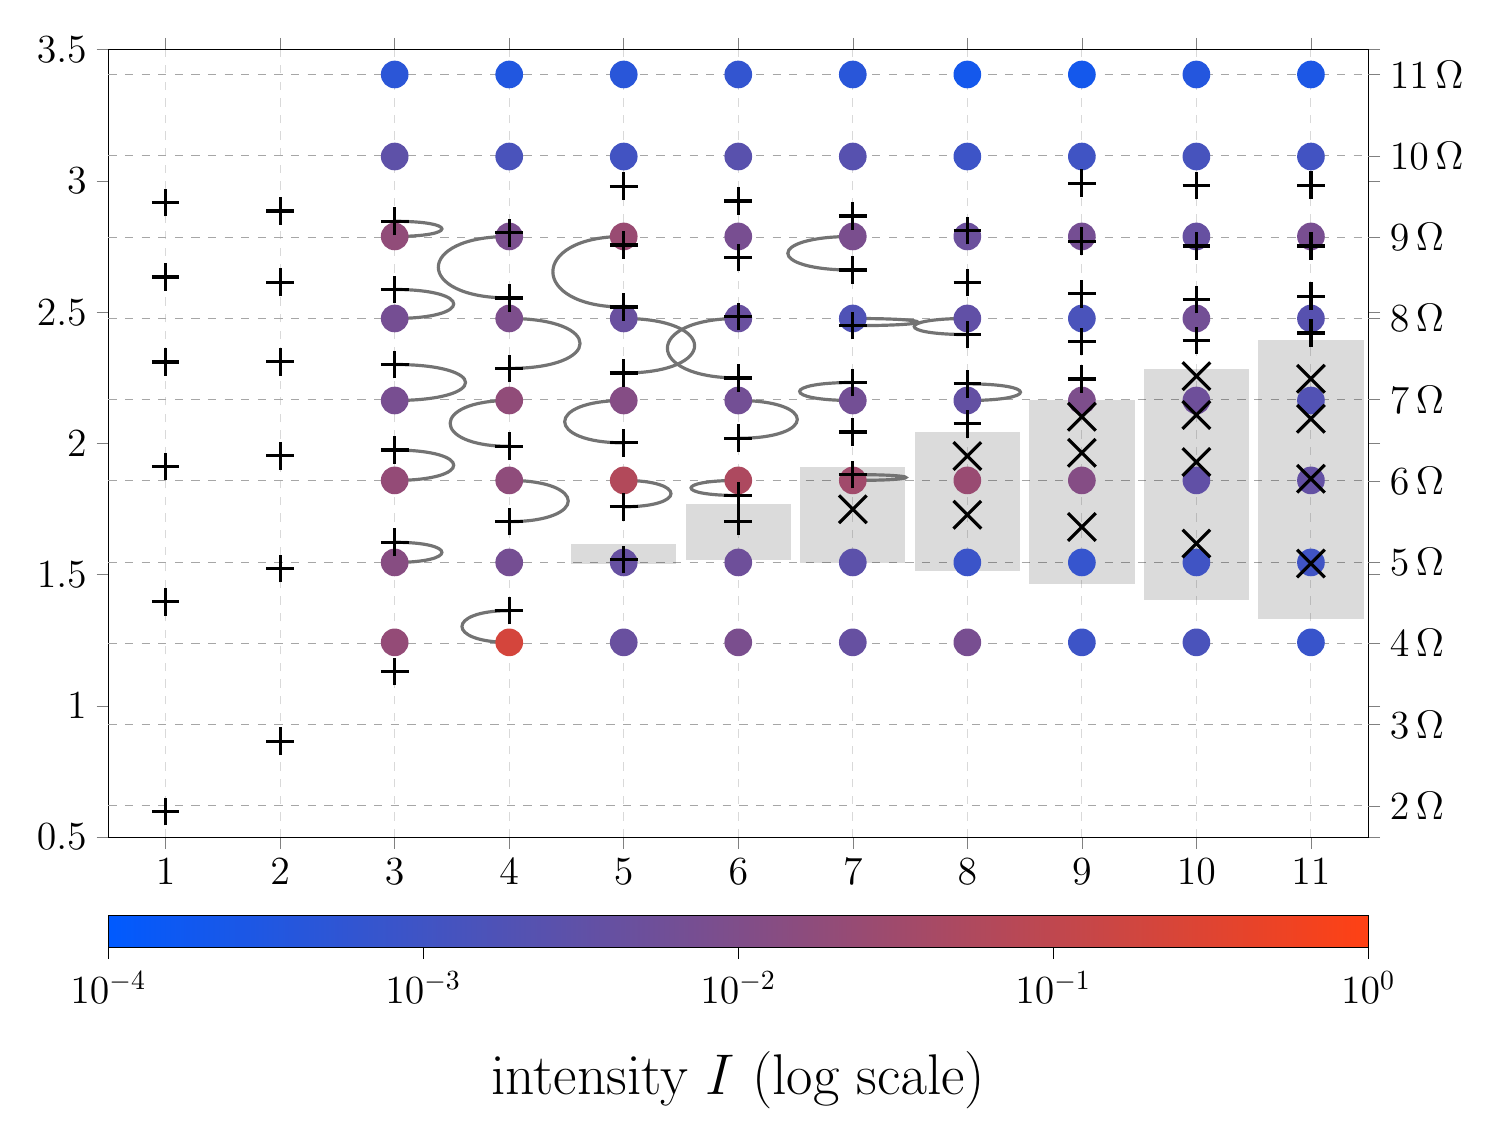
\begin{tikzpicture}[font=\PlotFont]

\begin{axis}[
  font=\PlotFont,
  scale only axis,
  width=\PlotWidth,
  height=\PlotHeight,
  xmin=\XMin,
  xmax=\XMax,
  ymin=\YMin,
  ymax=\YMax,
  axis lines=box,
  xtick={1,2,3,4,5,6,7,8,9,10,11},
  ytick distance=0.5,
  yticklabel pos=left,
  extra y ticks={
      0.619114228,
      0.928671341,
      1.238228455,
      1.547785569,
      1.857342683,
      2.166899797,
      2.476456911,
      2.786014024,
      3.095571138,
      3.405128252
  },
extra y tick labels={
      $2\,\Omega$,
      $3\,\Omega$,
      $4\,\Omega$,
      $5\,\Omega$,
      $6\,\Omega$,
      $7\,\Omega$,
      $8\,\Omega$,
      $9\,\Omega$,
      $10\,\Omega$,
      $11\,\Omega$
  },
  extra y tick style={
      tick pos=right,
      ticklabel pos=right,
      grid=none
  },
  tick align=outside,
  xmajorgrids=true,
  grid style={black!15,dashed},
  clip=false
]

% Exact lower corners of the plotting rectangle.
\coordinate (plotSW) at (rel axis cs:0,0);
\coordinate (plotSE) at (rel axis cs:1,0);

% ============================================================
% Guide levels: nu = k * CarrierNu
% ============================================================

\pgfmathtruncatemacro{\GuideFirst}{ceil(\YMin/\CarrierNu)}
\pgfmathtruncatemacro{\GuideLast}{floor(\YMax/\CarrierNu)}

\foreach \k in {\GuideFirst,...,\GuideLast} {

  \pgfmathsetmacro{\GuideY}{\k*\CarrierNu}

  \edef\GuideLine{%
    \noexpand\draw[
      GuideColor,
      dashed,
      line width=0.35pt
    ]
      (axis cs:\XMin,\GuideY)
      --
      (axis cs:\XMax,\GuideY);
  }

  \GuideLine
}

% ============================================================
% WKB / quasiclassical-limit bars
%
% Light rectangular bands centered at each m.
% Drawn behind correspondence arcs and point markers.
% ============================================================

\foreach \m/\nuMin/\nuMax in \WKBData {
  % Compute numeric left/right edges first.  Do not put arithmetic
  % expressions directly inside axis cs: coordinates.
  \pgfmathsetmacro{\WKBLeft}{\m-\WKBHalfWidth}
  \pgfmathsetmacro{\WKBRight}{\m+\WKBHalfWidth}

  \edef\ThisWKBBar{%
    \noexpand\path[
      fill=WKBColor,
      fill opacity=\WKBOpacity,
      draw=none
    ]
      (axis cs:\WKBLeft,\nuMin)
      rectangle
      (axis cs:\WKBRight,\nuMax);
  }
  \ThisWKBBar
}

% ============================================================
% Store experimental coordinates
% ============================================================

\foreach \m/\n/\nu/\intensity in \ExperimentData {

  \edef\StoreExperimentPoint{%
    \noexpand\coordinate
      (exp-\m-\n)
      at (axis cs:\m,\nu);
  }

  \StoreExperimentPoint
}

% ============================================================
% Store theoretical coordinates
% ============================================================

\foreach \m/\n/\nu/\flag/\mm/\nn in \TheoryData {

  \edef\StoreTheoryPoint{%
    \noexpand\coordinate
      (theo-\m-\n)
      at (axis cs:\m,\nu);
  }

  \StoreTheoryPoint
}

% ============================================================
% Correspondence arcs
%
% Each connection is controlled independently through \ArcData.
% The two Bezier control points are shifted by the same signed
% horizontal offset, producing a large, easy-to-read side arc.
% ============================================================

\foreach \tm/\tn/\xm/\xn/\offset in \ArcData {
  \edef\ThisArc{%
    \noexpand\DrawCorrespondenceArc
      {\tm}{\tn}{\xm}{\xn}{\offset}%
  }
  \ThisArc
}

% ============================================================
% Experimental circles
%
% log10(intensity) = -4.0        -> IntensityLow
% log10(intensity) = 0           -> IntensityHigh
% ============================================================

\foreach \m/\n/\nu/\intensity in \ExperimentData {

  \pgfmathtruncatemacro{\IntensityMix}{
    max(
      0,
      min(
        100,
        round(
          100*(\intensity-\IntensityMin)/
          (\IntensityMax-\IntensityMin)
        )
      )
    )
  }

  \edef\ThisExperimentPoint{%
    \noexpand\fill[
      fill=IntensityHigh!\IntensityMix!IntensityLow
    ]
      (exp-\m-\n)
      circle[radius=\CircleRadius];
  }

  \ThisExperimentPoint
}

% ============================================================
% Theory markers
%
% Drawn last -> always above experimental circles.
% ============================================================

\foreach \m/\n/\nu/\flag/\mm/\nn in \TheoryData {

  \edef\TheoryCoord{theo-\m-\n}
  \edef\TheoryFlag{\flag}

  \expandafter\DrawTheoryMarker
  \expandafter{\TheoryCoord}{\TheoryFlag}
}

\end{axis}

% ============================================================
% Intensity color bar
%
% Main axis uses "scale only axis", therefore the actual plotting
% rectangle width is exactly \PlotWidth.
% The colorbar therefore has exactly the same physical width.
% ============================================================

\coordinate (cbarSW)
  at ([yshift=-14mm]plotSW);

\coordinate (cbarSE)
  at ([xshift=\PlotWidth]cbarSW);

\coordinate (cbarNW)
  at ([yshift=4mm]cbarSW);

\coordinate (cbarNE)
  at ([xshift=\PlotWidth]cbarNW);

\shade[
  left color=IntensityLow,
  right color=IntensityHigh
]
  (cbarSW)
  rectangle
  (cbarNE);

\draw[
  black,
  line width=0.35pt
]
  (cbarSW)
  rectangle
  (cbarNE);

% Colorbar ticks. The data already contain log10(intensity),
% therefore tick positions are linear in log10(I), while the labels
% show the original intensity I.

\foreach \logI/\lab in {
  -4/{$10^{-4}$},
  -3/{$10^{-3}$},
  -2/{$10^{-2}$},
  -1/{$10^{-1}$},
  0/{$10^{0}$}
} {

  \pgfmathsetmacro{\fraction}{
    (\logI-\IntensityMin)/(\IntensityMax-\IntensityMin)
  }

  \coordinate (cbTick)
    at ($(cbarSW)!\fraction!(cbarSE)$);

  \draw[
    black,
    line width=0.35pt
  ]
    (cbTick)
    --
    ++(0,-1.5mm);

  \node[
    anchor=north
  ]
    at ($(cbTick)+(0,-1.8mm)$)
    {\lab};
}

\node[
  anchor=north,
  font=\PlotFont\scalefont{1.4}
]
  at ($(cbarSW)!0.5!(cbarSE)+(0,-12mm)$)
  {intensity $I$ (log scale)};

\end{tikzpicture}

\end{document}
